%!TEX root=../main.tex
% Chapter Template

\chapter{Design} % Main chapter title

\label{Chapter3} % Change X to a consecutive number; for referencing this chapter elsewhere, use \ref{ChapterX}

%----------------------------------------------------------------------------------------
%	SECTION 1
%----------------------------------------------------------------------------------------

\section{Conceptual overview of the system}
The system is developed as a part of the classic architectural pattern, Model-View-Controller (MVC) \cite{PatternsOfEnterprise}. The system itself consists of the Model and Controller part, and lets the client be responsible for the view, which in this case is the web shop. Figure \ref{fig:MVC} shows how the system is layered. Data is sent to the controller which simply communicates the data between the logic (model) of the system and the view. The logic (model) handles the data, instantiates objects and does calculations regarding product recommendations. \\
Apart from the MVC pattern the system has a persistence layer responsible for interactions with the database. The different layers communicate through interfaces in order to be able to substitute implementations in the future. 

\begin{figure}[H]
	\centering
	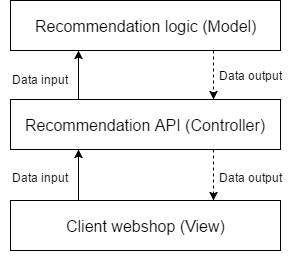
\includegraphics[width=.4\linewidth]{Figures/MVC.png}
	\caption{The Model-View-Controller (MVC) pattern applied on the system}
	\label{fig:MVC}
\end{figure}

\subsection{Recommendation API (Controller)}
The recommendation system is designed according to the MVC pattern described above. The controller layer takes input from the user (the web shop) and passes the information to the model layer. The controller layer is split into two classes, one for handling when the user requests recommendations which relates to functional requirement F01 and another for handling the data coming from the web shops relating to functional requirements F02-F15.

\subsection{Recommendation logic (Model)}
The recommendation logic is where the main operations of the system takes place. The model layer consists of five packages, and is made accessible to the controller layer through three interfaces. This layer consists of the entities seen in the domain model in Chapter \ref{analysis} as well as classes for handling the business logic. \\This is where the product recommendations are calculated before being sent back to the controller layer. This is also the package where any offline-calculation is made before it is stored in the database. The Entities and Utility package creates an easier and more manageable way of communicating data around within the model layer. All communication between the Controller-layer and the Model-layer is done through the interfaces seen in the Communication package. These interfaces are implemented by their corresponding classes in the Business and Persistence packages. The implementation of the Model-layer is discussed further in Chapter \ref{Chapter5}. \\
A package diagram of the Controller and Model layer as well as the persistence layer can be seen in figure \ref{fig:PackageDiagram}

\begin{figure}[H]
	\centering
	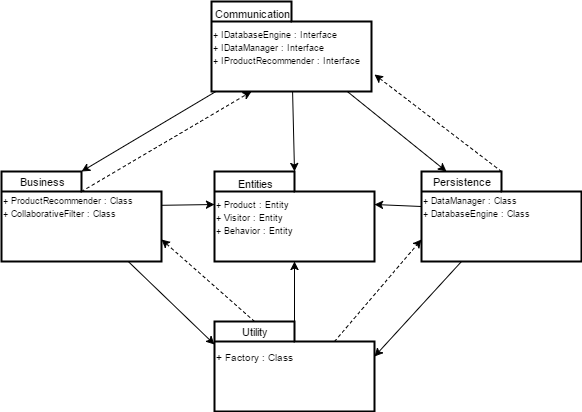
\includegraphics[width=.8\linewidth]{Figures/PackageDiagram.png}
	\caption{Package diagram of the model layer}
	\label{fig:PackageDiagram}
\end{figure}

\section{Client-Server}
When put to use, the recommendation system will be distributed and handle the server role in a Client-Server model. The system should be considered an application solely for providing product recommendations. In this scenario, the client is the web shop that needs to provide recommendations to one of its users. The client is also able to ask the server to update its database or store new content in the database, but the concept is the same and just as simple as the request for product recommendations. The Client-Server model of the system can be seen in figure \ref{fig:ClientServer}

\begin{figure}[H]
	\centering
	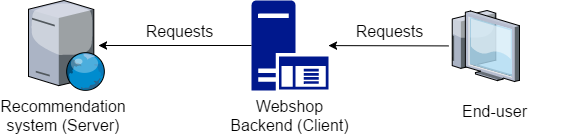
\includegraphics[width=.8\linewidth]{Figures/ClientServer.png}
	\caption{Package diagram of the model layer}
	\label{fig:ClientServer}
\end{figure}

\section{RESTfull}
RESTfull architectural style or SOAP messaging protocol can be used to accomplish requirement NF04 - Accessibility. RESTfull uses the HTTP protocol which defines GET, POST, PUT and DELETE methods for communication. REST is preferred over SOAP because it leverages less bandwidth \cite{restfull}. \\
REST is an acronym for REpresentational State Transfer and consists of five guiding constraints \cite{rest}:
\begin{description}
\item [Client-Server] By separating the concerns of user interface and data storage/manipulation we improve the portability of the user interface.
\item [Stateless] The server shall hold no state information about the client between requests.
\item [Cacheable] Responses shall be cacheable by the client.
\item [Uniform interface] The server shall present a uniform interface for interactions.
\item [Layered system] The system shall be layered.
\end{description}


\section{Database design}
Specific requirements for the storage of data was set by Struct, as they wanted a largely scalable structure of the data. The technology chosen was \gls{NoSQL}.
The data demands are not clearly specified in the beginning. No-SQL makes it easy to add or remove data or even change the data types. Traditional relational databases are rigid and have very strict data constraints. The flexible structure of No-SQL means that all data restrictions have to be handled in the code. The denormalized format of No-SQL allows for faster retrieval of a single item without having to do joins or complex SQL queries. Finally No-SQL is easier to scale across multiple servers and many engines have built in scaling functionalities which can come in handy when multiple clients begin using the service \cite{SQLvsNOSQL}. A downside of No-SQL compared to relational databases is the fact it does not focus much on Online Transaction Processing (OLTP) which means there is no guarantee that the data is always stored completely. Overall No-SQL is a good fit for this project since scalability and speed is imperative. \\\\

A brief overview of the different terminology for SQL and No-SQL is given in table \ref{sqlvsnosql_table}.
\begin{table}[H]
	\centering
	\caption{SQL vs No-SQL terminology}
	\label{sqlvsnosql_table}
	\begin{tabular}{|l|l|p{8cm}|}
		\hline
		\textbf{SQL}   & \textbf{No-SQL}     & \textbf{Comment}                                                                                                    \\ \hline
		Table & Collection &                                                                                                            \\ \hline
		Row   & Document   & A No-SQL document can contain more complex data types compared to a row in SQL e.g arrays or other documents \\
		\hline
	\end{tabular}
\end{table}

The database design mimics the domain model by representing real world concepts such as Products and, Visitors and their Behavior. The No-SQL design can be seen in figure \ref{documents}.

\begin{table}[H]
	\centering
	\caption{An overview of the fields in each document in the collections}
	\label{documents}
	\begin{tabular}{|l|l|p{7cm}|}
		\hline
		\textbf{Document} & \textbf{Fields}                                                                                                                          & \textbf{Comment}                                                                   \\ \hline
		Visitor           & \begin{tabular}[c]{@{}l@{}}Id\\ Behaviors\\ ProfileUID\\ CustomerUID\end{tabular}                         & The behavior array is an array of Behavior documents which contains all the behaviors of the specific visitor \\ \hline
		Product           & \begin{tabular}[c]{@{}l@{}}Id\\ ProductGroupId\\ VisitorId\\ Description\\ Created\end{tabular} &     The visitorId array contains Ids of all visitors who have looked at this product    \\ \hline
		Behavior & \begin{tabular}[c]{@{}l@{}}Type \\ Id \\ Timestamp \end{tabular} & A behavior document holds information about a particular view of a product.  \\ \hline
	\end{tabular}
\end{table}
